%%%%%%%%%%%%%%%%%%%%%%%%%%%%%%%%%%%%%%%%%%%%%%
% AI3603 Homework 1 Report
% Path Planning with A* Algorithm
%%%%%%%%%%%%%%%%%%%%%%%%%%%%%%%%%%%%%%%%%%%%%%
\documentclass[aps,letterpaper,10pt]{revtex4}

\usepackage{graphicx} % For images
\usepackage{float}    % For tables and other floats
\usepackage{verbatim} % For comments and other
\usepackage{amsmath}  % For math
\usepackage{amssymb}  % For more math
\usepackage{fullpage} % Set margins and place page numbers at bottom center
\usepackage{listings} % For source code
\usepackage{subfig}   % For subfigures
\usepackage[usenames,dvipsnames]{color} % For colors and names
\usepackage[pdftex]{hyperref}           % For hyperlinks and indexing the PDF
\usepackage{algorithm}
\usepackage{algpseudocode}

\hypersetup{
    colorlinks,
    citecolor=blue,
    filecolor=blue,
    linkcolor=blue,
    urlcolor=blue
}

\definecolor{mygrey}{gray}{.96}
\lstset{
	language=Python,
    tabsize=4,
	basicstyle=\small,
	numbers=left,
	numberstyle=\tiny,
	stepnumber=1,
	numbersep=5pt,
	backgroundcolor=\color{mygrey},
	frame=single,
	tabsize=4,
	captionpos=b,
	breaklines=true,
	breakatwhitespace=false,
	commentstyle=\color{BrickRed}
}

% TITLE PAGE CONTENT
\newcommand{\labtitle}{AI 3603 Artificial Intelligence: Principles and Techniques}
\newcommand{\authorname}{Mingxi Lyu (523030910081))}
\newcommand{\hw}{1}
\newcommand{\hwtitle}{Search Algorithm - Path Planning with A* Algorithm}

\begin{document}

% TITLE PAGE
\begin{titlepage}
\begin{center}
{\Large \textsc{\labtitle} \\ \vspace{4pt}}
\rule[13pt]{\textwidth}{1pt} \\ \vspace{80pt}
{\LARGE \textbf{Homework \hw} \\ \vspace{10pt}}
{\Large \hwtitle \\ \vspace{150pt}}
{\large By: \authorname \\ \vspace{10pt}
\today}
\end{center}
\end{titlepage}

%%%%%%%%%%%%%%%%%%%%%%%%%%%%%%
\section{Introduction}

This report presents the implementation and analysis of path planning algorithms for a service robot operating in a 2D environment. The assignment consists of three main tasks: implementing a basic A* algorithm, developing an improved A* algorithm with enhanced features, and creating a smooth path planner suitable for self-driving applications.

\subsection{Problem Statement}

Given a 120m $\times$ 120m world map discretized into a grid where each cell represents a 1.0m $\times$ 1.0m block, the objective is to plan an optimal path from a start position to a goal position while avoiding obstacles. The map is represented as a 120 $\times$ 120 array where 0 indicates traversable space and 1 indicates obstacles.

\subsection{Objectives}

The three main objectives of this homework are:

\begin{enumerate}
    \item \textbf{Task 1}: Implement a basic A* algorithm with 4-directional movement (forward, backward, left, right)
    \item \textbf{Task 2}: Develop an improved A* algorithm incorporating:
    \begin{itemize}
        \item 8-directional movement (including diagonals)
        \item Obstacle distance consideration for safety
        \item Steering cost to reduce unnecessary turns
    \end{itemize}
    \item \textbf{Task 3}: Create a smooth path planner for self-driving applications using path smoothing techniques
\end{enumerate}

%%%%%%%%%%%%%%%%%%%%%%%%%%%%%%
\newpage
\section{Task 1: Basic A* Algorithm}

\subsection{Algorithm Description}

The A* algorithm is a best-first search algorithm that finds the optimal path from a start node to a goal node. It uses a heuristic function to guide the search and guarantees finding the shortest path when using an admissible heuristic.

\subsection{Mathematical Formulation}

The A* algorithm evaluates nodes using the cost function:

\begin{equation}
f(n) = g(n) + h(n)
\end{equation}

where:
\begin{itemize}
    \item $f(n)$ is the total estimated cost of the path through node $n$
    \item $g(n)$ is the actual cost from the start node to node $n$
    \item $h(n)$ is the heuristic estimated cost from node $n$ to the goal
\end{itemize}

For Task 1, the Manhattan distance heuristic is used:

\begin{equation}
h(n) = |x_n - x_g| + |y_n - y_g|
\end{equation}

where $(x_n, y_n)$ is the position of node $n$ and $(x_g, y_g)$ is the goal position.

\subsection{Implementation Details}

\textbf{Movement Model}: The robot can move in 4 directions with unit cost:
\begin{itemize}
    \item Right: $(0, 1)$
    \item Left: $(0, -1)$
    \item Down: $(1, 0)$
    \item Up: $(-1, 0)$
\end{itemize}

\textbf{Data Structures}:
\begin{itemize}
    \item \texttt{open\_list}: Priority queue (min-heap) storing nodes to be explored
    \item \texttt{closed\_set}: Set of already explored nodes
    \item \texttt{g\_scores}: Dictionary tracking the best known cost to reach each position
\end{itemize}

\textbf{Algorithm Steps}:
\begin{enumerate}
    \item Initialize start node with $g=0$, $h=h(\text{start}, \text{goal})$, $f=g+h$
    \item Add start node to open list
    \item While open list is not empty:
    \begin{enumerate}
        \item Pop node with lowest $f$ score
        \item If node is goal, reconstruct and return path
        \item Add node to closed set
        \item For each valid neighbor:
        \begin{enumerate}
            \item Calculate $g$, $h$, and $f$ scores
            \item If neighbor offers better path, add to open list
        \end{enumerate}
    \end{enumerate}
    \item If open list is empty, no path exists
\end{enumerate}

\subsection{Results}

Figure \ref{fig:task1} shows the path generated by the basic A* algorithm. The path successfully navigates from the start position (10, 10) to the goal position (100, 100) while avoiding all obstacles.

\begin{figure}[H]
  \centering
  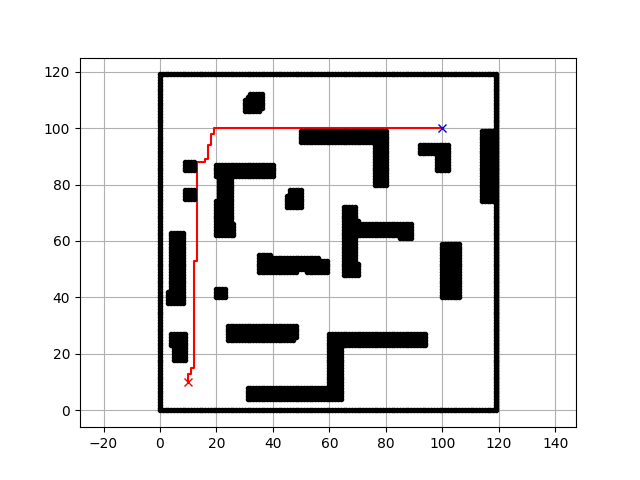
\includegraphics[width=0.7\textwidth]{assets/task-1.png}
  \caption{Path generated by basic A* algorithm with 4-directional movement. The red line shows the planned path, red 'x' marks the start position, and blue 'x' marks the goal position.}
  \label{fig:task1}
\end{figure}

\textbf{Observations}:
\begin{itemize}
    \item The path consists of only horizontal and vertical segments
    \item The algorithm finds an optimal path in terms of grid distance
    \item The path exhibits a staircase pattern due to 4-directional movement constraint
    \item Computational efficiency is good due to the admissible heuristic
\end{itemize}

%%%%%%%%%%%%%%%%%%%%%%%%%%%%%%
\newpage
\section{Task 2: Improved A* Algorithm}

\subsection{Algorithm Description}

The improved A* algorithm extends the basic version with three key enhancements to produce safer and more efficient paths suitable for real-world robotic applications.

\subsection{Enhancements}

\subsubsection{8-Directional Movement}

The movement model is extended to include diagonal movements:

\textbf{Orthogonal movements} (cost = 1.0):
\begin{itemize}
    \item Right: $(0, 1)$, Left: $(0, -1)$, Down: $(1, 0)$, Up: $(-1, 0)$
\end{itemize}

\textbf{Diagonal movements} (cost = $\sqrt{2} \approx 1.414$):
\begin{itemize}
    \item Down-right: $(1, 1)$, Down-left: $(1, -1)$
    \item Up-right: $(-1, 1)$, Up-left: $(-1, -1)$
\end{itemize}

The Euclidean distance heuristic is used for better accuracy:

\begin{equation}
h(n) = \sqrt{(x_n - x_g)^2 + (y_n - y_g)^2}
\end{equation}

\subsubsection{Obstacle Distance Consideration}

To maintain safe distance from obstacles, a distance transform is computed using the Euclidean Distance Transform (EDT). The obstacle penalty is:

\begin{equation}
P_{\text{obs}}(n) = \begin{cases}
w_{\text{obs}} \cdot (d_{\text{min}} - d(n)) & \text{if } d(n) < d_{\text{min}} \\
0 & \text{otherwise}
\end{cases}
\end{equation}

where:
\begin{itemize}
    \item $d(n)$ is the distance from node $n$ to the nearest obstacle
    \item $d_{\text{min}} = 3.0$ is the minimum safe distance
    \item $w_{\text{obs}} = 2.0$ is the obstacle distance weight
\end{itemize}

\subsubsection{Steering Cost}

To reduce unnecessary turns and create smoother paths, a steering cost is added based on the change in direction. The steering cost is calculated using the dot product of direction vectors:

\begin{equation}
P_{\text{steer}}(n) = w_{\text{steer}} \cdot \left(1 - \frac{\vec{d}_{\text{prev}} \cdot \vec{d}_{\text{new}}}{|\vec{d}_{\text{prev}}| \cdot |\vec{d}_{\text{new}}|}\right) \cdot 0.5
\end{equation}

where:
\begin{itemize}
    \item $\vec{d}_{\text{prev}}$ is the direction vector from parent to current node
    \item $\vec{d}_{\text{new}}$ is the direction vector from current to neighbor node
    \item $w_{\text{steer}} = 5.0$ is the steering weight
    \item The dot product term equals 1 for same direction, 0 for 90°, -1 for opposite direction
\end{itemize}

\subsection{Modified Cost Function}

The total cost function for the improved A* is:

\begin{equation}
g(n) = g(\text{parent}) + c_{\text{move}} + P_{\text{obs}}(n) + P_{\text{steer}}(n)
\end{equation}

where $c_{\text{move}}$ is 1.0 for orthogonal moves and $\sqrt{2}$ for diagonal moves.

\subsection{Results}

Figure \ref{fig:task2} shows the path generated by the improved A* algorithm.

\begin{figure}[H]
  \centering
  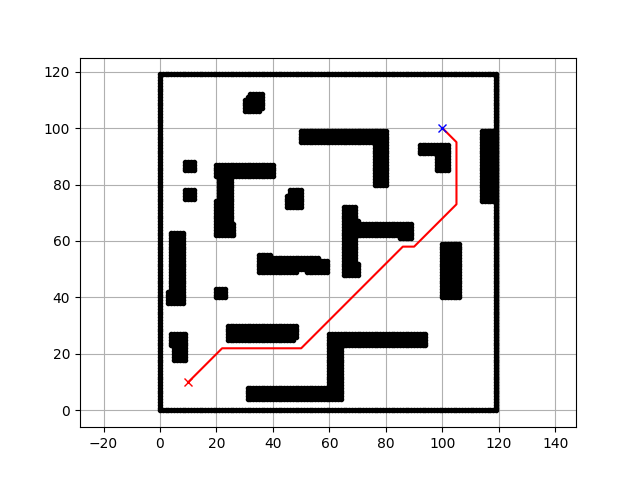
\includegraphics[width=0.7\textwidth]{assets/task-2.png}
  \caption{Path generated by improved A* algorithm with 8-directional movement, obstacle avoidance, and steering cost. The path is smoother with fewer turns and maintains safe distance from obstacles.}
  \label{fig:task2}
\end{figure}

\textbf{Observations}:
\begin{itemize}
    \item The path uses diagonal movements, resulting in a more direct route
    \item Fewer waypoints compared to Task 1 due to diagonal movements
    \item The path maintains a safe distance from obstacles
    \item Reduced number of direction changes due to steering cost penalty
    \item More natural and efficient path suitable for robotic navigation
\end{itemize}

%%%%%%%%%%%%%%%%%%%%%%%%%%%%%%
\newpage
\section{Task 3: Self-Driving Path Planner}

\subsection{Algorithm Description}

The self-driving path planner builds upon the improved A* algorithm and adds path smoothing to create continuous, smooth trajectories suitable for autonomous vehicles. The smoothing process ensures comfort and energy efficiency.

\subsection{Three-Stage Approach}

\subsubsection{Stage 1: Initial Path Generation}

The improved A* algorithm from Task 2 is used to generate an initial path with:
\begin{itemize}
    \item 8-directional movement
    \item Obstacle distance consideration
    \item Steering cost to reduce turns
\end{itemize}

\subsubsection{Stage 2: Path Simplification}

The initial path is simplified by removing redundant waypoints that do not significantly change the path direction. This is done by analyzing the angle between consecutive path segments.

For three consecutive points $p_{i-1}$, $p_i$, $p_{i+1}$, the point $p_i$ is kept if:

\begin{equation}
\vec{v}_1 \cdot \vec{v}_2 < (1 - \theta_{\text{threshold}})
\end{equation}

where:
\begin{itemize}
    \item $\vec{v}_1 = \frac{p_i - p_{i-1}}{|p_i - p_{i-1}|}$ (normalized vector)
    \item $\vec{v}_2 = \frac{p_{i+1} - p_i}{|p_{i+1} - p_i|}$ (normalized vector)
    \item $\theta_{\text{threshold}} = 0.1$ (angle threshold)
\end{itemize}

This removes collinear points while preserving key turning points.

\subsubsection{Stage 3: B-Spline Smoothing}

A cubic B-spline interpolation is applied to create a smooth, continuous curve. The B-spline is parameterized by:

\begin{equation}
\mathbf{C}(u) = \sum_{i=0}^{n} N_{i,k}(u) \mathbf{P}_i, \quad u \in [0, 1]
\end{equation}

where:
\begin{itemize}
    \item $\mathbf{P}_i$ are the control points (simplified waypoints)
    \item $N_{i,k}(u)$ are the B-spline basis functions
    \item $k = 3$ for cubic splines
    \item $s = 2.0$ is the smoothing parameter (allows slight deviation from waypoints)
\end{itemize}

The spline is evaluated at 200 uniformly distributed parameter values to generate a dense, smooth path.

\subsection{Path Validation}

After smoothing, the path is validated to ensure it does not collide with obstacles. Each point is checked:

\begin{enumerate}
    \item Verify the point is within map bounds
    \item Verify the point is in free space (not an obstacle)
    \item If more than 20\% of points are invalid, revert to original path
\end{enumerate}

\subsection{Implementation Details}

\textbf{Key Functions}:
\begin{itemize}
    \item \texttt{improved\_a\_star\_base()}: Generates initial path using improved A*
    \item \texttt{simplify\_path()}: Removes redundant waypoints
    \item \texttt{smooth\_path\_with\_spline()}: Applies B-spline smoothing
    \item \texttt{validate\_and\_fix\_path()}: Ensures collision-free path
\end{itemize}

\textbf{Parameters}:
\begin{itemize}
    \item Angle threshold for simplification: 0.1
    \item Number of interpolation points: 200
    \item Spline smoothing factor: 2.0
    \item Spline degree: 3 (cubic)
\end{itemize}

\subsection{Results}

Figure \ref{fig:task3} shows the smooth path generated for self-driving applications.

\begin{figure}[H]
  \centering
  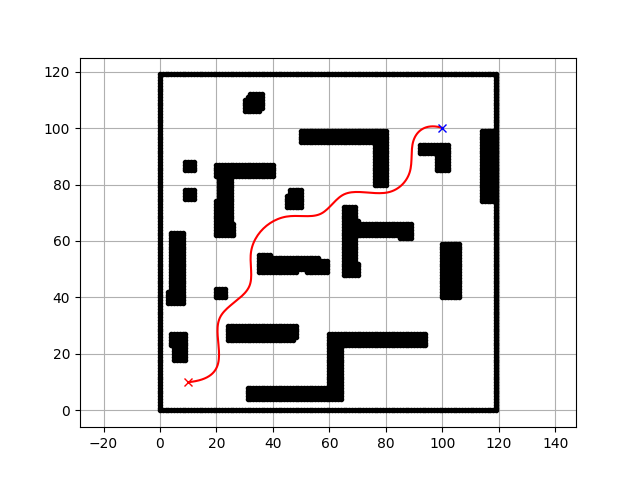
\includegraphics[width=0.7\textwidth]{assets/task-3.png}
  \caption{Smooth path generated by the self-driving path planner using B-spline interpolation. The path is continuous and smooth, suitable for autonomous vehicle navigation.}
  \label{fig:task3}
\end{figure}

\textbf{Observations}:
\begin{itemize}
    \item The path is smooth and continuous with no sharp corners
    \item Suitable for vehicles with kinematic constraints
    \item Maintains safe distance from obstacles
    \item Provides comfortable trajectory for passengers
    \item Energy-efficient due to smooth acceleration and steering
    \item The dense sampling (200 points) ensures fine-grained control
\end{itemize}

%%%%%%%%%%%%%%%%%%%%%%%%%%%%%%
\newpage
\section{Comparison and Analysis}

\subsection{Qualitative Comparison}

Table \ref{tab:comparison} summarizes the key differences between the three approaches.

\begin{table}[H]
\begin{center}
\begin{tabular}{|l|c|c|c|}
\hline
\textbf{Feature} & \textbf{Task 1} & \textbf{Task 2} & \textbf{Task 3} \\ \hline
Movement Directions & 4 & 8 & 8 \\ \hline
Path Smoothness & Low & Medium & High \\ \hline
Obstacle Safety & Basic & Enhanced & Enhanced \\ \hline
Turn Optimization & No & Yes & Yes \\ \hline
Continuity & Discrete & Discrete & Continuous \\ \hline
Self-Driving Ready & No & Partial & Yes \\ \hline
\end{tabular}
\end{center}
\caption{Comparison of the three path planning approaches}
\label{tab:comparison}
\end{table}

\subsection{Path Characteristics}

\textbf{Task 1 - Basic A*}:
\begin{itemize}
    \item \textbf{Pros}: Simple, guaranteed optimal for grid, fast computation
    \item \textbf{Cons}: Staircase pattern, many waypoints, not smooth, frequent turns
    \item \textbf{Use Case}: Grid-based robots, simple navigation
\end{itemize}

\textbf{Task 2 - Improved A*}:
\begin{itemize}
    \item \textbf{Pros}: More direct paths, safer (obstacle distance), fewer turns, more efficient
    \item \textbf{Cons}: Still discrete, not perfectly smooth
    \item \textbf{Use Case}: Mobile robots, warehouse automation, general robotics
\end{itemize}

\textbf{Task 3 - Self-Driving Planner}:
\begin{itemize}
    \item \textbf{Pros}: Smooth and continuous, comfortable, energy-efficient, suitable for vehicles
    \item \textbf{Cons}: More complex, requires validation, slightly longer computation time
    \item \textbf{Use Case}: Autonomous vehicles, self-driving cars, applications requiring smooth motion
\end{itemize}

\subsection{Computational Complexity}

\textbf{Time Complexity}:
\begin{itemize}
    \item \textbf{Task 1 \& 2}: $O(b^d)$ where $b$ is the branching factor (4 or 8) and $d$ is the depth
    \item With priority queue: $O(E \log V)$ where $E$ is edges and $V$ is vertices
    \item \textbf{Task 3}: Additional $O(n)$ for simplification and $O(n^2)$ for spline fitting
\end{itemize}

\textbf{Space Complexity}:
\begin{itemize}
    \item All tasks: $O(V)$ for storing nodes in open and closed lists
    \item Task 2 \& 3: Additional $O(V)$ for distance transform
\end{itemize}

\subsection{Safety Analysis}

The obstacle distance consideration in Tasks 2 and 3 significantly improves safety:

\begin{itemize}
    \item Minimum safe distance of 3.0 units from obstacles
    \item Distance transform provides gradient information
    \item Paths naturally avoid narrow passages when safer alternatives exist
    \item Validation step in Task 3 ensures smoothed path remains collision-free
\end{itemize}

\subsection{Optimality}

\textbf{Task 1}: Guarantees optimal path in terms of grid distance (Manhattan metric)

\textbf{Task 2}: Near-optimal with respect to Euclidean distance, but trades pure optimality for safety and smoothness

\textbf{Task 3}: Sacrifices strict optimality for smoothness and continuity, which is more important for real-world vehicle applications

%%%%%%%%%%%%%%%%%%%%%%%%%%%%%%
\newpage
\section{Discussion}

\subsection{Implementation Challenges}

\subsubsection{Heuristic Selection}

Choosing the appropriate heuristic function was crucial. Manhattan distance works well for 4-directional movement (Task 1) as it is admissible and consistent. For 8-directional movement (Tasks 2 \& 3), Euclidean distance provides better estimates and leads to fewer node expansions.

\subsubsection{Parameter Tuning}

The improved A* algorithm requires careful tuning of several parameters:

\begin{itemize}
    \item \textbf{Obstacle distance weight} ($w_{\text{obs}} = 2.0$): Too low results in paths too close to obstacles; too high causes excessive detours
    \item \textbf{Steering weight} ($w_{\text{steer}} = 5.0$): Balances between path length and smoothness
    \item \textbf{Minimum safe distance} ($d_{\text{min}} = 3.0$): Based on robot size and safety requirements
\end{itemize}

The steering weight was adjusted from the initial value of 1.5 to 5.0 to achieve better turn reduction while maintaining reasonable path length.

\subsubsection{Spline Smoothing}

B-spline smoothing presented several challenges:

\begin{itemize}
    \item \textbf{Degree selection}: Cubic splines (degree 3) provide good smoothness while avoiding oscillations
    \item \textbf{Smoothing factor}: $s = 2.0$ allows slight deviation from waypoints for smoother curves
    \item \textbf{Validation}: Essential to ensure smoothed path doesn't cut through obstacles
    \item \textbf{Fallback mechanism}: Returns original path if smoothing fails or creates collisions
\end{itemize}

\subsection{Advantages of the Approach}

\begin{enumerate}
    \item \textbf{Progressive Enhancement}: Each task builds upon the previous, allowing modular development
    \item \textbf{Safety-Aware}: Obstacle distance consideration prevents dangerous paths
    \item \textbf{Practical}: The final solution is suitable for real-world autonomous vehicles
    \item \textbf{Flexible}: Parameters can be tuned for different robot types and environments
    \item \textbf{Robust}: Validation and fallback mechanisms ensure reliability
\end{enumerate}

\subsection{Potential Improvements}

\subsubsection{Dynamic Environments}

The current implementation assumes a static environment. For dynamic obstacles, the algorithm could be extended with:
\begin{itemize}
    \item D* or D* Lite for replanning
    \item Time dimension in the state space
    \item Velocity obstacles for moving obstacle avoidance
\end{itemize}

\subsubsection{Kinematic Constraints}

For real vehicles, additional constraints should be considered:
\begin{itemize}
    \item Maximum turning radius
    \item Maximum acceleration and deceleration
    \item Velocity limits
    \item Hybrid A* or State Lattice approaches
\end{itemize}

\subsubsection{Multi-Objective Optimization}

The cost function could be extended to optimize multiple objectives:
\begin{itemize}
    \item Energy consumption
    \item Travel time
    \item Passenger comfort
    \item Pareto-optimal solutions
\end{itemize}

\subsubsection{Alternative Smoothing Methods}

Other smoothing techniques could be explored:
\begin{itemize}
    \item Polynomial interpolation (simpler but may oscillate)
    \item Bezier curves (good local control)
    \item Clothoid curves (constant curvature change)
    \item Optimization-based smoothing (e.g., gradient descent)
\end{itemize}

%%%%%%%%%%%%%%%%%%%%%%%%%%%%%%
\section{Conclusion}

This homework successfully implemented three progressively sophisticated path planning algorithms for robotic navigation. The basic A* algorithm (Task 1) provides optimal grid-based paths with 4-directional movement. The improved A* algorithm (Task 2) enhances the basic version with 8-directional movement, obstacle distance consideration, and steering cost optimization, resulting in safer and more efficient paths. The self-driving path planner (Task 3) adds B-spline smoothing to create continuous, smooth trajectories suitable for autonomous vehicles.

The comparison analysis demonstrates clear improvements across the three tasks in terms of path quality, safety, and suitability for real-world applications. While Task 1 is optimal for simple grid navigation, Task 3 provides the smooth, continuous paths required for passenger comfort and energy efficiency in self-driving vehicles.

Key achievements include:
\begin{itemize}
    \item Successful implementation of A* with proper heuristics
    \item Integration of safety considerations through distance transforms
    \item Effective turn reduction through steering cost penalties
    \item Smooth path generation using B-spline interpolation
    \item Robust validation mechanisms to ensure collision-free paths
\end{itemize}

The progressive approach from basic to advanced algorithms provides valuable insights into the trade-offs between optimality, safety, smoothness, and computational complexity in path planning. The final self-driving planner represents a practical solution that balances these factors for real-world autonomous navigation applications.

Future work could explore dynamic replanning, kinematic constraints, and multi-objective optimization to further enhance the path planning capabilities for complex real-world scenarios.

\end{document}

